\documentclass[12pt]{article}
\usepackage[paper=letterpaper,margin=2cm]{geometry}
\usepackage{amsmath}
\usepackage{amssymb}
\usepackage{amsfonts}
\usepackage{newtxtext, newtxmath}
\usepackage{enumitem}
\usepackage{titling}
\usepackage{svg}
\usepackage{xcolor}
\usepackage{listings}
\usepackage{float}
\usepackage{multicol}
\usepackage{nicefrac}
\usepackage{ragged2e}
\usepackage[autostyle]{csquotes}
\usepackage[colorlinks=true]{hyperref}

\MakeOuterQuote{"}
\setlength{\droptitle}{-6em}

\definecolor{codegreen}{rgb}{0,0.6,0}
\definecolor{codegray}{rgb}{0.5,0.5,0.5}
\definecolor{codepurple}{rgb}{0.58,0,0.82}
\definecolor{backcolour}{rgb}{0.95,0.95,0.92}

\lstdefinestyle{mystyle}{
    commentstyle=\color{codegreen},
    keywordstyle=\color{magenta},
    numberstyle=\tiny\color{codegray},
    stringstyle=\color{codepurple},
    basicstyle=\ttfamily\footnotesize,
    breakatwhitespace=false,
    breaklines=true,
    captionpos=b,
    keepspaces=true,
    numbers=left,
    numbersep=5pt,
    showspaces=false,
    showstringspaces=false,
    showtabs=false,
    tabsize=2
}

\lstset{
        style=mystyle,
        inputencoding=utf8,
        extendedchars=true,
}


\title{\large{Aprendizagem 2022}\vskip 0.2cm Homework III -- Group 019\vskip 0.2cm Diogo Gaspar 99207, Rafael Oliveira 99311}
\date{}
\begin{document}
\maketitle
\center\large{\vskip -2.5cm\textbf{Part I}: Pen and paper}
\begin{enumerate}[leftmargin=\labelsep]

  \item \textbf{Consider the basis function, $\phi_j(x) = x^j$, for performing a 3-order polynomial regression,
          $$
            \hat{z}(x, w) = \sum_{j=0}^3 w_j \phi_j(x) = w_0 + w_1 x + w_2 x^2 + w_3 x^3.
          $$
          Learn the Ridge regression ($l_2$ regularization) on the transformed data space
          using the closed-form solution with $\lambda = 2$.
        }

        We have in hands a \textbf{supervised learning} problem, with a given training
        dataset as shown below:

        \begin{table}[h]
          \centering
          \begin{tabular}{c|c|c}
                  & $y_1$ & $z$  \\ \hline
            $x_1$ & $0.8$ & $24$ \\
            $x_2$ & $1$   & $20$ \\
            $x_3$ & $1.2$ & $10$ \\
            $x_4$ & $1.4$ & $13$ \\
            $x_5$ & $1.6$ & $12$
          \end{tabular}
          \caption{Training dataset: $y_1$ as the input's (only) variable, $z$ as the target variable}
          \label{tab:training-dataset}
        \end{table}

        We can note that in the statement's estimation function, $\hat{z}(x, w)$, $x$ is a single-element vector
        (with its only entry being each sample's $y_1$ value). Therefore, it makes
        sense to "expand" the table above as follows, in order to have a broader
        representation of the values we'll end up using in the estimation function:

        \begin{table}[h]
          \centering
          \begin{tabular}{c|ccc|c}
                  & $y_1$ & $y_1^2$ & $y_1^3$ & $z$  \\ \hline
            $x_1$ & $0.8$ & $0.64$  & $0.512$ & $24$ \\
            $x_2$ & $1$   & $1$     & $1$     & $20$ \\
            $x_3$ & $1.2$ & $1.44$  & $1.728$ & $10$ \\
            $x_4$ & $1.4$ & $1.96$  & $2.744$ & $13$ \\
            $x_5$ & $1.6$ & $2.56$  & $4.096$ & $12$
          \end{tabular}
          \caption{Training dataset with additional information}
          \label{tab:expanded-training-dataset}
        \end{table}

        The equation below shows the closed-form solution for the Ridge regression
        problem, with $\lambda = 2$:

        \begin{equation*}
          % account for lambda, the bias term
          w = (\Phi^T \Phi + \lambda I)^{-1} \Phi^T z = (\Phi^T \Phi + 2 I)^{-1} \Phi^T z
        \end{equation*}

        Here, $\Phi$ is the result of applying the basis function to our training
        dataset's inputs, such that:

        \begin{equation*}
          \Phi = \begin{bmatrix}
            1      & \phi_1(x_1) & \phi_2(x_1) & \phi_3(x_1) \\
            1      & \phi_1(x_2) & \phi_2(x_2) & \phi_3(x_2) \\
            \vdots & \vdots      & \vdots      & \vdots      \\
            1      & \phi_1(x_5) & \phi_2(x_5) & \phi_3(x_5)
          \end{bmatrix} = \begin{bmatrix}
            1 & 0.8 & 0.64 & 0.512 \\
            1 & 1   & 1    & 1     \\
            1 & 1.2 & 1.44 & 1.728 \\
            1 & 1.4 & 1.96 & 2.744 \\
            1 & 1.6 & 2.56 & 4.096
          \end{bmatrix}
        \end{equation*}

        We are now able to learn the given polynomial regression model, with $\lambda = 2$:
        $$
          \begin{aligned}
            (\Phi^T \Phi + \lambda I)^{-1} & = \left(
            \begin{bmatrix}
              1 & 0.8 & 0.64 & 0.512 \\
              1 & 1   & 1    & 1     \\
              1 & 1.2 & 1.44 & 1.728 \\
              1 & 1.4 & 1.96 & 2.744 \\
              1 & 1.6 & 2.56 & 4.096
            \end{bmatrix}^T
            \begin{bmatrix}
              1 & 0.8 & 0.64 & 0.512 \\
              1 & 1   & 1    & 1     \\
              1 & 1.2 & 1.44 & 1.728 \\
              1 & 1.4 & 1.96 & 2.744 \\
              1 & 1.6 & 2.56 & 4.096
            \end{bmatrix} +
            \begin{bmatrix}
              2 & 0 & 0 & 0 \\
              0 & 2 & 0 & 0 \\
              0 & 0 & 2 & 0 \\
              0 & 0 & 0 & 2
            \end{bmatrix}
            \right)^{-1}                                                                             \\
                                           & = \begin{bmatrix}
                                                 0.34168753  & -0.1214259  & -0.07490231 & -0.00932537 \\
                                                 -0.1214259  & 0.3892078   & -0.09667718 & -0.07445624 \\
                                                 -0.07490231 & -0.09667718 & 0.37257788  & -0.17135047 \\
                                                 -0.00932537 & -0.07445624 & -0.17135047 & 0.17998796  \\
                                               \end{bmatrix}
          \end{aligned}
        $$

        \begin{equation*}
          \Phi^T z = \begin{bmatrix}
            1 & 0.8 & 0.64 & 0.512 \\
            1 & 1   & 1    & 1     \\
            1 & 1.2 & 1.44 & 1.728 \\
            1 & 1.4 & 1.96 & 2.744 \\
            1 & 1.6 & 2.56 & 4.096
          \end{bmatrix}^T
          \begin{bmatrix}
            24 \\
            20 \\
            10 \\
            13 \\
            12
          \end{bmatrix} = \begin{bmatrix}
            79      \\
            88.6    \\
            105.96  \\
            134.392 \\
          \end{bmatrix}
        \end{equation*}

        \begin{equation*}
          w = (\Phi^T \Phi + \lambda I)^{-1} \Phi^T z = \begin{bmatrix}
            7.0450759   \\
            4.64092765  \\
            1.96734046  \\
            -1.30088142 \\
          \end{bmatrix}
        \end{equation*}

        Having learned the regression model, we can now use it to predict labels $z$
        for new samples!

        \pagebreak

  \item \textbf{Compute the training RMSE for the learnt regression model.}

        We know that the Root Mean Squared Error (RMSE) for a given regression model is
        defined as

        \begin{equation*}
          \text{RMSE} = \sqrt{\frac{1}{N} \sum_{i=1}^N (z_i - \hat{z}_i)^2},
        \end{equation*}

        where $N$ is the number of samples in the dataset, $z_i$ is the true label for
        the $i$-th sample, and $\hat{z}_i$ is the predicted label for the $i$-th sample.
        As stated in the previous question's statement, $\hat{z}$ is given by the matrix product
        $\Phi \cdot w$. We can, then, compute the RMSE for the training dataset as follows:

        \begin{equation*}
          \begin{aligned}
            \hat{z} = \Phi \cdot w & = \begin{bmatrix}
                                         1 & 0.8 & 0.64 & 0.512 \\
                                         1 & 1   & 1    & 1     \\
                                         1 & 1.2 & 1.44 & 1.728 \\
                                         1 & 1.4 & 1.96 & 2.744 \\
                                         1 & 1.6 & 2.56 & 4.096
                                       \end{bmatrix}
            \begin{bmatrix}
              7.0450759   \\
              4.64092765  \\
              1.96734046  \\
              -1.30088142 \\
            \end{bmatrix} = \begin{bmatrix}
                              11.35086463 \\
                              12.35246259 \\
                              13.19923625 \\
                              13.8287433  \\
                              14.17854143 \\
                            \end{bmatrix}                                                                                    \\
            \text{RMSE}            & = \sqrt{\frac{1}{5} \sum_{i=1}^5 (z_i - \hat{z}_i)^2}                                    \\
                                   & = \sqrt{\frac{1}{5} \left( (24 - 11.35086463)^2 + \hdots + (12 - 14.17854143)^2 \right)} \\
                                   & = 6.84329
          \end{aligned}
        \end{equation*}

        \pagebreak

  \item \textbf{Consider a multi-layer perceptron characterized by one hidden layer with 2 nodes.
          Using the activation function $f(x) = e^{0.1x}$ on all units, all weights
          initialized as 1 (including biases), and the half squared error loss, perform
          one batch gradient descent update (with learning rate $\eta = 0.1$)
          for the first three observations (0.8), (1) and (1.2).
        }

        Our multi-layer perceptron, considering the parameters stated above, should only
        have one output-node, since we're considering a regression problem aiming to
        predict a single output variable. As such, we can represent the network as follows:

        \begin{figure}[H]
          \centering
          \includesvg{../assets/hw3-3-mlp-shape.svg}
          \caption{Multi-layer perceptron shape}
        \end{figure}

        Each node in the hidden layer has an activation function $f(x) = e^{0.1x}$.
        Moreover, we know that the learning rule for the weights of the hidden layer
        is given by $\Delta w = - \eta \frac{\partial E}{\partial w}$ (with an analogous
        logic associated to biases), with $\eta = 0.1$ and $E$ being the half squared error loss.

        \begin{equation*}
          E = \frac{1}{2 * 2} \sum_{i=1}^N (z_i - \hat{z}_i)^2
        \end{equation*}

        A gradient descent update will require us to go through 3 phases: forward
        propagation, back propagation and updates (via gradient updates, updating
        biases and weights).

        Starting by the forward propagation, and considering $l$ as a given layer,
        we have that:

        \begin{equation*}
          z^{(l)} = w^{(l)} x^{(l - 1)} + b^{(l)}, \quad x^{(l)} = f(z^{(l)})
        \end{equation*}

        \pagebreak

        We also know, from the question's statement, both the input nodes' values
        and weight/bias matrices:

        \begin{equation*}
          \begin{aligned}
            x^{(0)} & = \begin{bmatrix}
                          0.8 \\
                          1   \\
                          1.2
                        \end{bmatrix}, \quad
            w^{(1)} & = \begin{bmatrix}
                          1 & 1 & 1 \\
                          1 & 1 & 1
                        \end{bmatrix}, \quad
            b^{(1)} & = \begin{bmatrix}
                          1 \\
                          1
                        \end{bmatrix}, \quad
            w^{(2)} & = \begin{bmatrix}
                          1 & 1
                        \end{bmatrix}, \quad
            b^{(2)} & = \begin{bmatrix}
                          1
                        \end{bmatrix}
          \end{aligned}
        \end{equation*}

        Applying the afore-mentioned equations in succession will lead us to the following results:


        % FIXME: align second members
        \begin{equation*}
          \begin{aligned}
            z^{(1)} & = \begin{bmatrix}
                          4.00000000 \\
                          4.00000000
                        \end{bmatrix}, \quad
                    &                      & x^{(1)} = \begin{bmatrix}
                                                         1.4918247 \\
                                                         1.4918247
                                                       \end{bmatrix} \\
            z^{(2)} & = \begin{bmatrix}
                          3.9836494 \\
                        \end{bmatrix}, \quad
                    &                      & x^{(2)} = \begin{bmatrix}
                                                         1.48938747
                                                       \end{bmatrix}
          \end{aligned}
        \end{equation*}

        We're now ready for the back propagation phase. Applying batch gradient descent,
        and looking at the half squared error loss, we have that:

        \begin{equation*}
          \Delta w^{[l]} = - \eta \frac{\partial E}{\partial w^{[l]}}, \quad
          \Delta b^{[l]} = - \eta \frac{\partial E}{\partial b^{[l]}}
        \end{equation*}

        We'll want to propagate information backwards; for that, we'll need to use
        the chain rule, multiplying successive derivatives as we go backwards.
        With $L$ being the \textbf{last layer} - will be useful for reusing previously
        calculated $\delta$'s - we have the following equalities:

        \begin{align*}
          \frac{\partial E}{\partial w^{[L]}} & = \textcolor{teal}{\frac{\partial E}{\partial x^{[L]}} \circ
            \frac{\partial x^{[L]}}{\partial z^{[L]}}}
          \frac{\partial z^{[L]^T}}{\partial w^{[L]}}                                                        \\
          \frac{\partial E}{\partial b^{[L]}} & = \textcolor{teal}{\frac{\partial E}{\partial x^{[L]}} \circ
            \frac{\partial x^{[L]}}{\partial z^{[L]}}}
          \frac{\partial z^{[L]^T}}{\partial b^{[L]}}                                                        \\
          \delta^{[L]}                        & = \textcolor{teal}{\frac{\partial E}{\partial x^{[L]}} \circ
          \frac{\partial x^{[L]}}{\partial z^{[L]}}}                                                         \\
          \delta^{[l]}                        & =
          \frac{\partial z^{[l + 1]^T}}{\partial x^{[l]}} \cdot \delta^{[l + 1]} \circ \frac{\partial x^{[l]}}{\partial z^{[l]}}
        \end{align*}

        \pagebreak

        We'll now be able to start propagating backwards (considering the following equalities,
        derived both in class and in the curricular unit's book):

        % derivative of the error loss

        \begin{equation*}
          \begin{aligned}
            \frac{\partial E}{\partial x^{[2]}} = \frac{\partial \frac{1}{4}\sum_{i=1}^N (z_i - x_i^{[2]})^2}{\partial x^{[2]}} = \frac{x^{[2]} - z_i}{2}, \quad
            \frac{\partial x^{[l]}}{\partial z^{[l]}} = \frac{\partial e^{0.1z^{[l]}}}{\partial z^{[l]}} = 0.1e^{0.1z^{[l]}}
          \end{aligned}
        \end{equation*}

        \begin{equation*}
          \begin{aligned}
            \frac{\partial z^{[l]}}{\partial x^{[l - 1]}} = w^{[l]}, \quad
            \frac{\partial z^{[l]}}{\partial b^{[l]}} = 1, \quad
            \frac{\partial z^{[l]}}{\partial w^{[l]}} = x^{[l - 1]}
          \end{aligned}
        \end{equation*}

        \begin{multicols}{2}
          \setlength{\columnseprule}{1pt}
          \def\columnseprulecolor{\color{black}}
          \centering

          \begin{equation*}
            \begin{aligned}
              \textcolor{purple}{\delta^{[2]}} & = \textcolor{teal}{\frac{\partial E}{\partial x^{[2]}} \circ
              \frac{\partial x^{[2]}}{\partial z^{[2]}}}                                                               \\
                                               & = \frac{(x^{[2]} - z_i)}{2} \circ 0.1e^{0.1z^{[2]}}                   \\
                                               & = \begin{bmatrix}
                                                     0.244693735
                                                   \end{bmatrix} \circ \begin{bmatrix} 0.1e^{0.39836494} \end{bmatrix} \\
                                               & = \begin{bmatrix}
                                                     0.03644437824
                                                   \end{bmatrix}
            \end{aligned}
          \end{equation*}

          \columnbreak

          \begin{equation*}
            \begin{aligned}
              \textcolor{purple}{\delta^{[1]}} & = \frac{\partial z^{[2]^T}}{\partial x^{[1]}} \cdot \delta^{[2]} \circ \frac{\partial x^{[1]}}{\partial z^{[1]}} \\
                                               & = \begin{bmatrix}
                                                     0.03644437824 \\
                                                     0.03644437824
                                                   \end{bmatrix} \circ \begin{bmatrix}
                                                                         0.1 e^{0.4} \\
                                                                         0.1 e^{0.4}
                                                                       \end{bmatrix}                                                                             \\
                                               & = \begin{bmatrix}
                                                     0.005436862355 \\
                                                     0.005436862355
                                                   \end{bmatrix}
            \end{aligned}
          \end{equation*}

        \end{multicols}

        In the last phase, we'll be updating our model: after computing the gradients,
        we'll be able to update weights and biases!

        Starting with weight matrices:

        \begin{equation*}
          \frac{\partial E}{\partial w^{[1]}} = \delta^{[1]} \cdot
          \frac{\partial z^{[1]^T}}{\partial w^{[1]}}
          = \delta^{[1]} \cdot x^{[0]^T}
          = \begin{bmatrix}
            0.00434949 & 0.00543686 & 0.00652423 \\
            0.00434949 & 0.00543686 & 0.00652423 \\
          \end{bmatrix}
        \end{equation*}

        \begin{equation*}
          \frac{\partial E}{\partial w^{[2]}} = \delta^{[2]} \cdot
          \frac{\partial z^{[2]^T}}{\partial w^{[2]}}
          = \delta^{[2]}
          \cdot x^{[1]^T}
          = \begin{bmatrix}
            0.05436862 & 0.05436862 \\
          \end{bmatrix}
        \end{equation*}

        \begin{equation*}
          \begin{aligned}
            w^{[1]} = w^{[1]} - \eta \cdot \frac{\partial E}{\partial w^{[1]}}
             & = \begin{bmatrix}
                   1 & 1 & 1 \\
                   1 & 1 & 1
                 \end{bmatrix} - 0.1 \cdot \begin{bmatrix}
                                             0.00434949 & 0.00543686 & 0.00652423 \\
                                             0.00434949 & 0.00543686 & 0.00652423 \\
                                           \end{bmatrix} \\
             & = \begin{bmatrix}
                   0.999565051 & 0.999456314 & 0.999347577 \\
                   0.999565051 & 0.999456314 & 0.999347577 \\
                   0.999565051 & 0.999456314 & 0.999347577
                 \end{bmatrix}
          \end{aligned}
        \end{equation*}

        \begin{equation*}
          \begin{aligned}
            w^{[2]} = w^{[2]} - \eta \cdot \frac{\partial E}{\partial w^{[2]}}
             & = \begin{bmatrix}
                   1 & 1
                 \end{bmatrix} - 0.1 \cdot \begin{bmatrix}
                                             0.05436862 & 0.05436862 \\
                                           \end{bmatrix} \\
             & = \begin{bmatrix}
                   0.994563138 & 0.994563138
                 \end{bmatrix}
          \end{aligned}
        \end{equation*}

        After updating weights, we'll update biases:

        \begin{equation*}
          \frac{\partial E}{\partial b^{[1]}} = \delta^{[1]} \cdot
          \frac{\partial z^{[1]^T}}{\partial b^{[1]}}
          = \delta^{[1]} \cdot 1
          = \delta^{[1]}
          = \begin{bmatrix}
            0.00543686 \\
            0.00543686 \\
          \end{bmatrix}
        \end{equation*}

        \begin{equation*}
          \frac{\partial E}{\partial b^{[2]}} = \delta^{[2]} \cdot
          \frac{\partial z^{[2]^T}}{\partial b^{[2]}}
          = \delta^{[2]} \cdot 1
          = \delta^{[2]}
          = \begin{bmatrix}
            0.03644438 \\
          \end{bmatrix}
        \end{equation*}

        \begin{equation*}
          \begin{aligned}
            b^{[1]} = b^{[1]} - \eta \cdot \frac{\partial E}{\partial b^{[1]}}
             & = \begin{bmatrix}
                   1 \\
                   1
                 \end{bmatrix} - 0.1 \cdot \begin{bmatrix}
                                             0.00543686 \\
                                             0.00543686 \\
                                           \end{bmatrix} \\
             & = \begin{bmatrix}
                   0.99945631 \\
                   0.99945631 \\
                 \end{bmatrix}
          \end{aligned}
        \end{equation*}

        \begin{equation*}
          \begin{aligned}
            b^{[2]} = b^{[2]} - \eta \cdot \frac{\partial E}{\partial b^{[2]}}
             & = \begin{bmatrix}
                   1
                 \end{bmatrix} - 0.1 \cdot \begin{bmatrix}
                                             0.03644438 \\
                                           \end{bmatrix} \\
             & = \begin{bmatrix}
                   0.99635556 \\
                 \end{bmatrix}
          \end{aligned}
        \end{equation*}

        % TODO: thingies

\end{enumerate}

\pagebreak

\center\large{\textbf{Part II}: Programming and critical analysis}

\begin{justify}
  The code utilized to answer the following questions is available in this
  report's appendix.
\end{justify}

\begin{enumerate}[leftmargin=\labelsep,resume]
  \item \textbf{Compute the MAE of the three regressors: linear regression, $MLP_1$ and $MLP_2$.}

        We opted to utilize \texttt{sklearn}'s \texttt{mean\_absolute\_error} function to compute the MAE of the three regressors.
        The regressors were created as shown in the appendix (using \texttt{Ridge} and
        \texttt{MLPRegressor} with the respective parameters).

        We gathered the following results:

        \begin{table}[h]
          \centering
          \begin{tabular}{l|l}
            Regressor                 & MAE       \\ \hline
            Linear Regression (Ridge) & $0.16283$ \\
            $MLP_1$                   & $0.06804$ \\
            $MLP_2$                   & $0.09781$
          \end{tabular}
          \caption{Gathered Mean Absolute Errors for each specified regressor}
          \label{tab:mean-absolute-errors}
        \end{table}

  \item \textbf{Plot the residues (in absolute value) using two visualizations: boxplots and histograms.}

        Each regressor's residues, calculated as the absolute difference between
        the predicted and actual values, were plotted using both boxplots and histograms
        (using, respectively, \texttt{seaborn}'s \texttt{boxplot} and \texttt{histplot} functions),
        as shown in this report's appendix (figure after the code).

  \item \textbf{How many iterations were required for $MLP_1$ and $MLP_2$ to converge?}

        Calling the \texttt{print\_regressor} method for each regressor shows us
        not only the MAE, but also the number of iterations required for each of
        the MLP regressors to converge. In this case, the number of iterations
        required for $MLP_1$ ($MLP$ with early stopping) to converge was 452,
        while $MLP_2$ ($MLP$ \textit{without} early stopping) required only 77.

  \item \textbf{What can be motivating the unexpected differences on the number of iterations?
          Hypothetize one reason underlying the observed performance differences between the MLPs.}

        As has been noted in the previous question's answer, $MLP_1$ takes many more
        iterations to converge than $MLP_2$ - almost six times as many. It's probably
        worth emphasizing that the number of iterations in a batch gradient descent
        algorithm matches the number of epochs ran - the amount of times the algorithm goes
        through the entire dataset. Early stopping, however, is a technique which
        allows us to \textbf{stop an epoch} at a given point, not the entire algorithm.

        % TODO: reasons for the difference in iterations

        Regarding performance, we were able to assert in the first question's answer
        that $MLP_1$ performed better than $MLP_2$ - it had a lower MAE, which
        effectively tells us that it was able to better approximate the function
        we were trying to learn to the data. With $MLP_1$ utilizing early stopping,
        it's likely that the regressor was able to avoid overfitting the data
        a bit better than $MLP_2$ - stopping at the "right point" of an epoch, instead
        of running the algorithm for all samples, could allow it to generalize
        better to unseen data.


\end{enumerate}

\pagebreak

\large{\textbf{Appendix}\vskip 0.3cm}

\lstinputlisting[language=Python]{code.py}

% TODO: figures should be presented neatly, currently aren't

\begin{figure}[H]
  \centering
  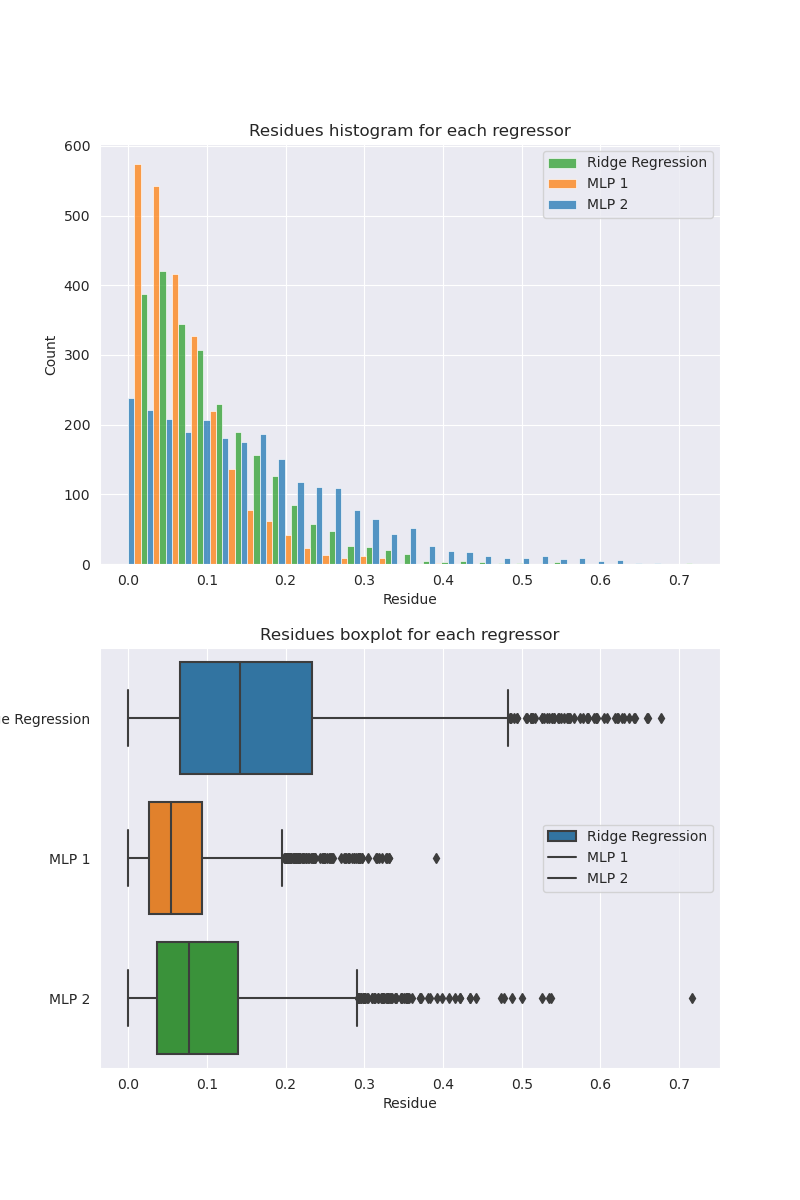
\includegraphics[width=\textwidth]{../assets/residues.png}
  \caption{Ridge regression's residue plotting}
  \label{fig:residue-plotting}
\end{figure}

\end{document}
